\clearpage
\section{软件架构 UML 图}

共绘制 6 张 UML 图：结构性的类图与组件图，行为性的用例图、活动图与状态图，交互性的时序图。全部使用 PlantUML 编写，源码随交付物提交。

\subsection{结构性图（一）：类图}

\begin{center}
\begin{minipage}{\textwidth}\centering
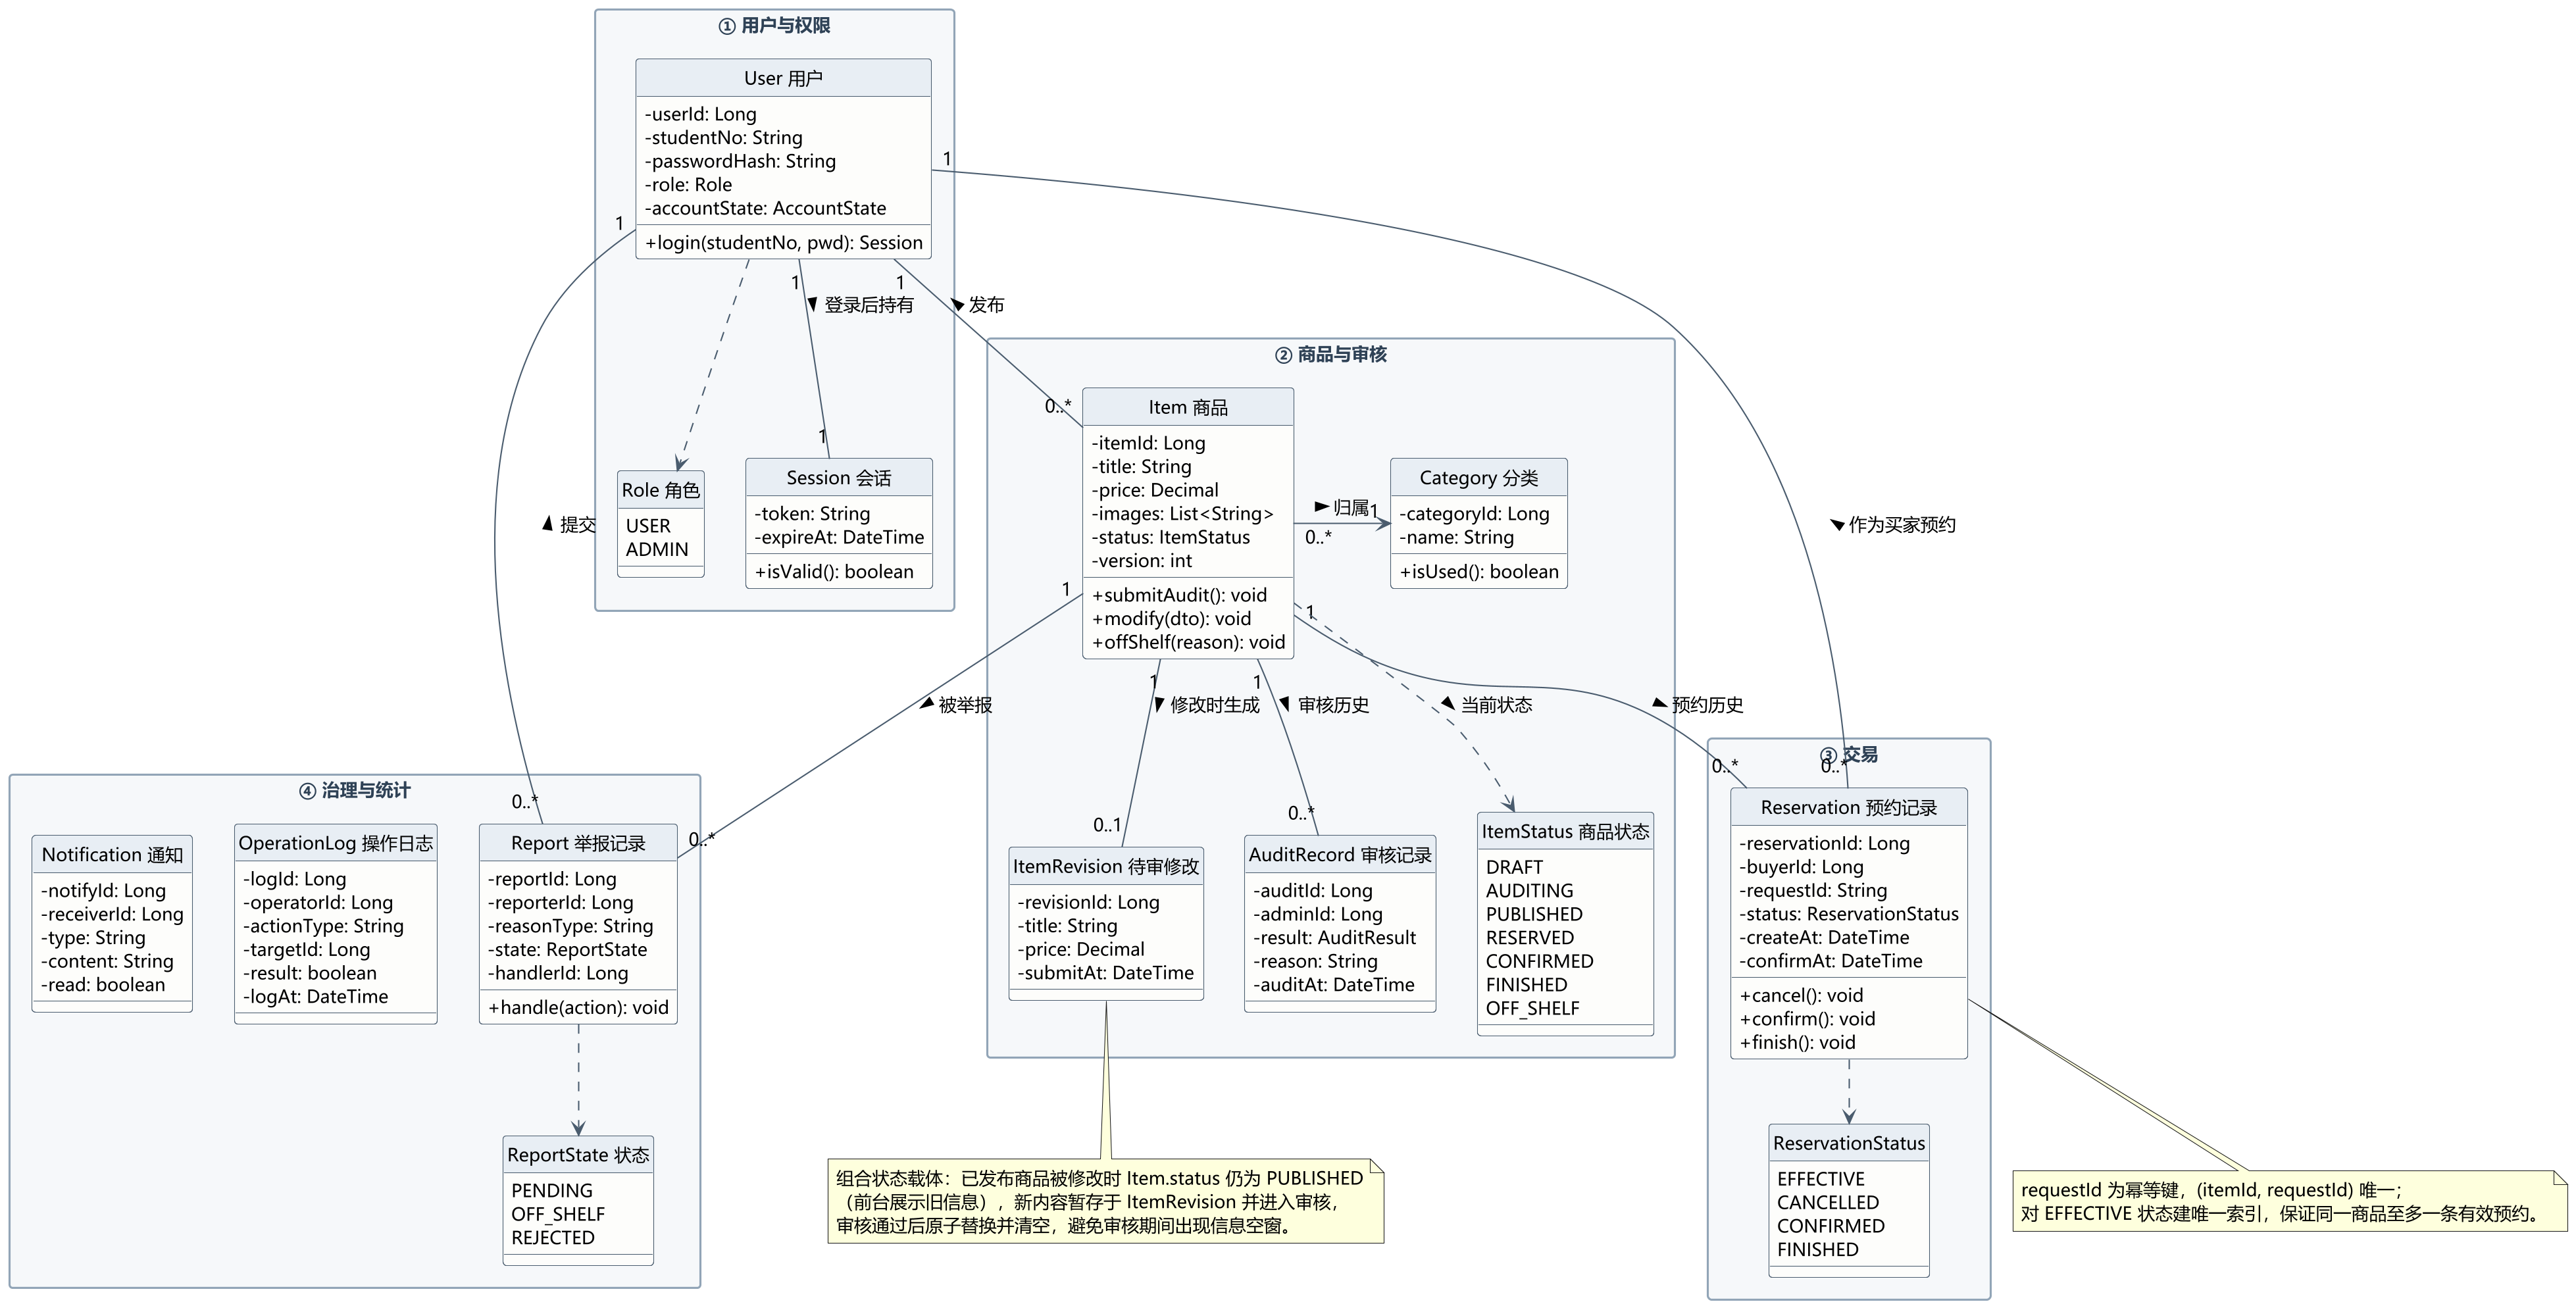
\includegraphics[width=0.99\textwidth]{uml1.png}
\par\vspace{2pt}
\captionof{figure}{校园二手交易系统类图}\label{fig:uml1}
\end{minipage}
\end{center}

类图按用户与权限、商品与审核、交易、治理与统计四个包组织，共 14 个类与枚举。三个关键设计：

\begin{enumerate}[leftmargin=2em,itemsep=1pt]
  \item \textbf{Item 与 ItemRevision 是组合关系}。已发布商品被修改时 Item.status 仍为 PUBLISHED（前台展示旧信息），新内容暂存 ItemRevision 等待审核，通过后原子替换。这是 REQ-017 组合状态在结构上的落点，也解释了“审核期间仍可预约”。
  \item \textbf{实体只暴露状态流转方法}。Item 只有 submitAudit()、modify()、offShelf()，没有 setStatus()，任何状态变更都必须经过校验，从结构上堵住绕过规则改状态。
  \item \textbf{Reservation 携带幂等键 requestId}。商品与预约是一对多，但有效预约唯一；多重性写在连线上会误导实现，因此用注释说明：数据库对 (item\_id, request\_id) 与“状态为 EFFECTIVE 时取 item\_id 的生成列”各建唯一索引，前者保证重复提交不重复创建，后者保证同一商品至多一条有效预约。
\end{enumerate}

\clearpage
\subsection{结构性图（二）：组件图}

\begin{center}
\begin{minipage}{\textwidth}\centering
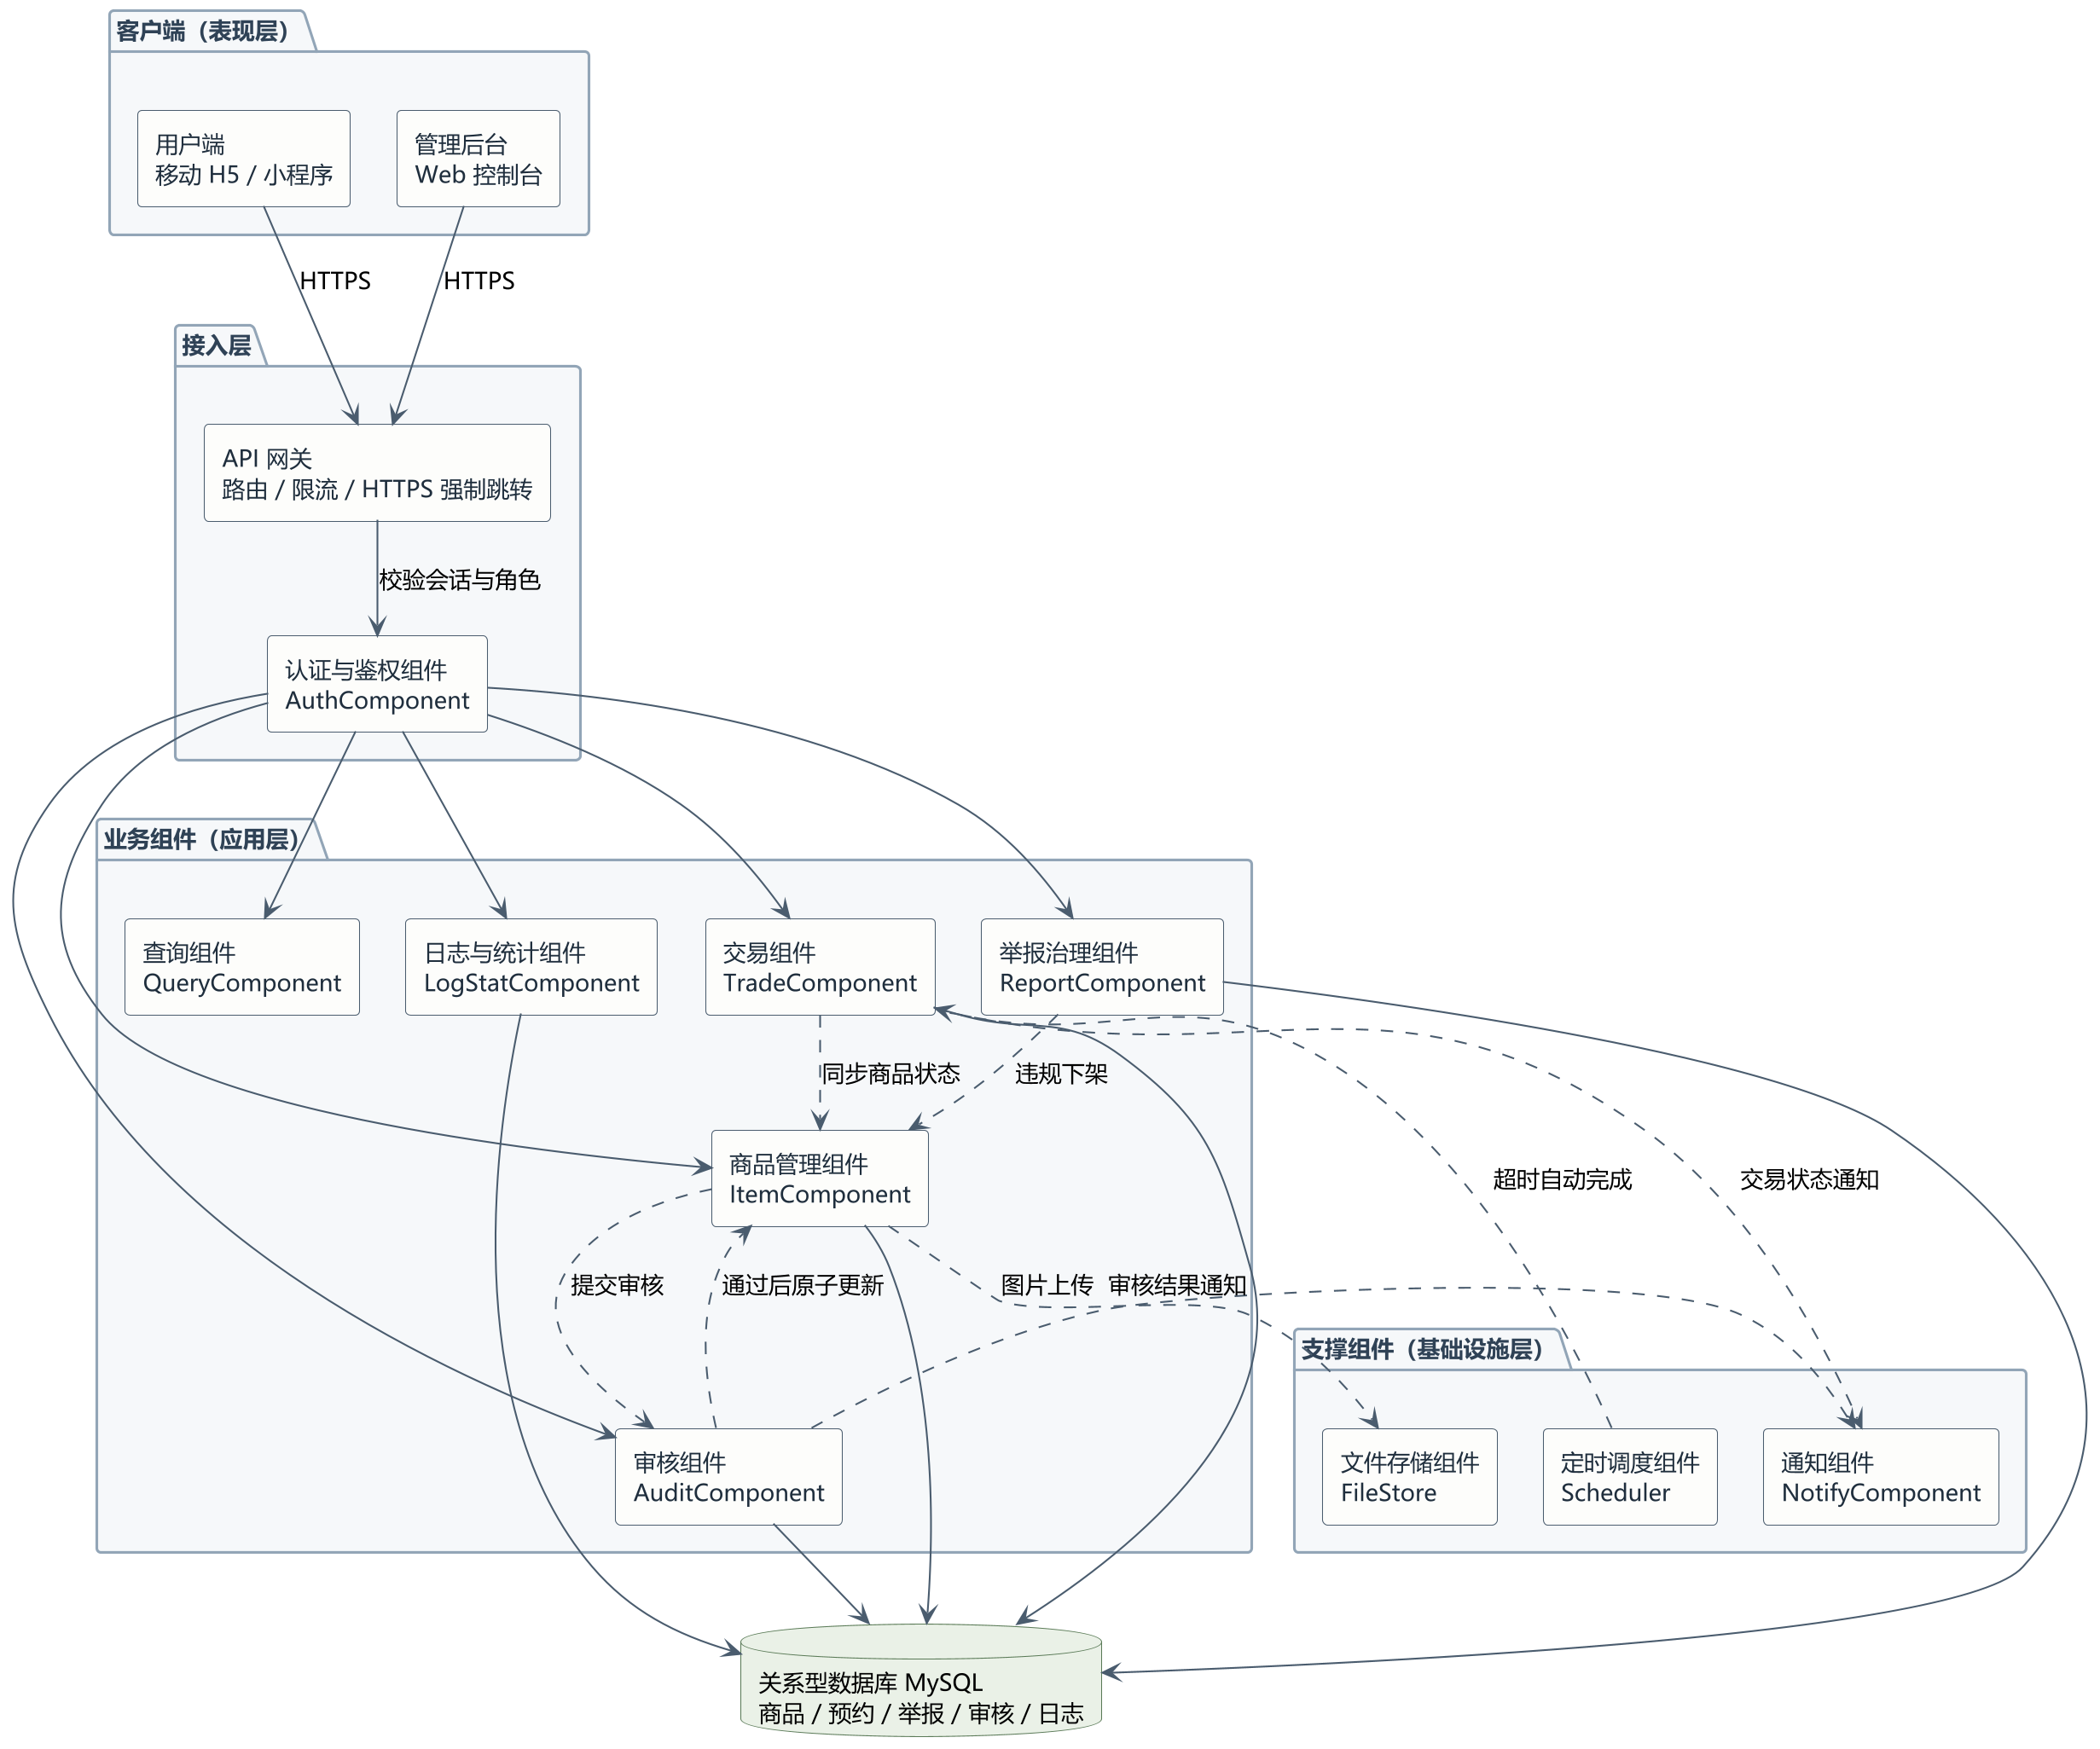
\includegraphics[width=0.88\textwidth]{uml2.png}
\par\vspace{2pt}
\captionof{figure}{校园二手交易系统组件图}\label{fig:uml2}
\end{minipage}
\end{center}

组件图把系统切成客户端、接入层、业务组件、支撑组件四层。客户端只通过 HTTPS 访问 API 网关，网关负责路由、限流与强制跳转 HTTPS（REQ-012），鉴权组件统一校验会话与角色后才分发到业务组件；支撑组件提供通知、定时调度与文件存储，其中定时调度是 REQ-015 超时自动完成的唯一入口。

这样分层的原因是需求中存在大量“状态同步”：预约、审核、举报下架都要改商品状态。如果每个组件都能直接写商品表，一致性只能靠人工保证；组件图用“交易组件 $\rightarrow$ 商品管理组件：同步商品状态”这条依赖说明，状态只有商品组件能写，其他组件只能请求它写。这既是模块边界，也是后续拆分部署的依据。

\clearpage
\subsection{行为性图（一）：用例图}

\begin{center}
\begin{minipage}{\textwidth}\centering
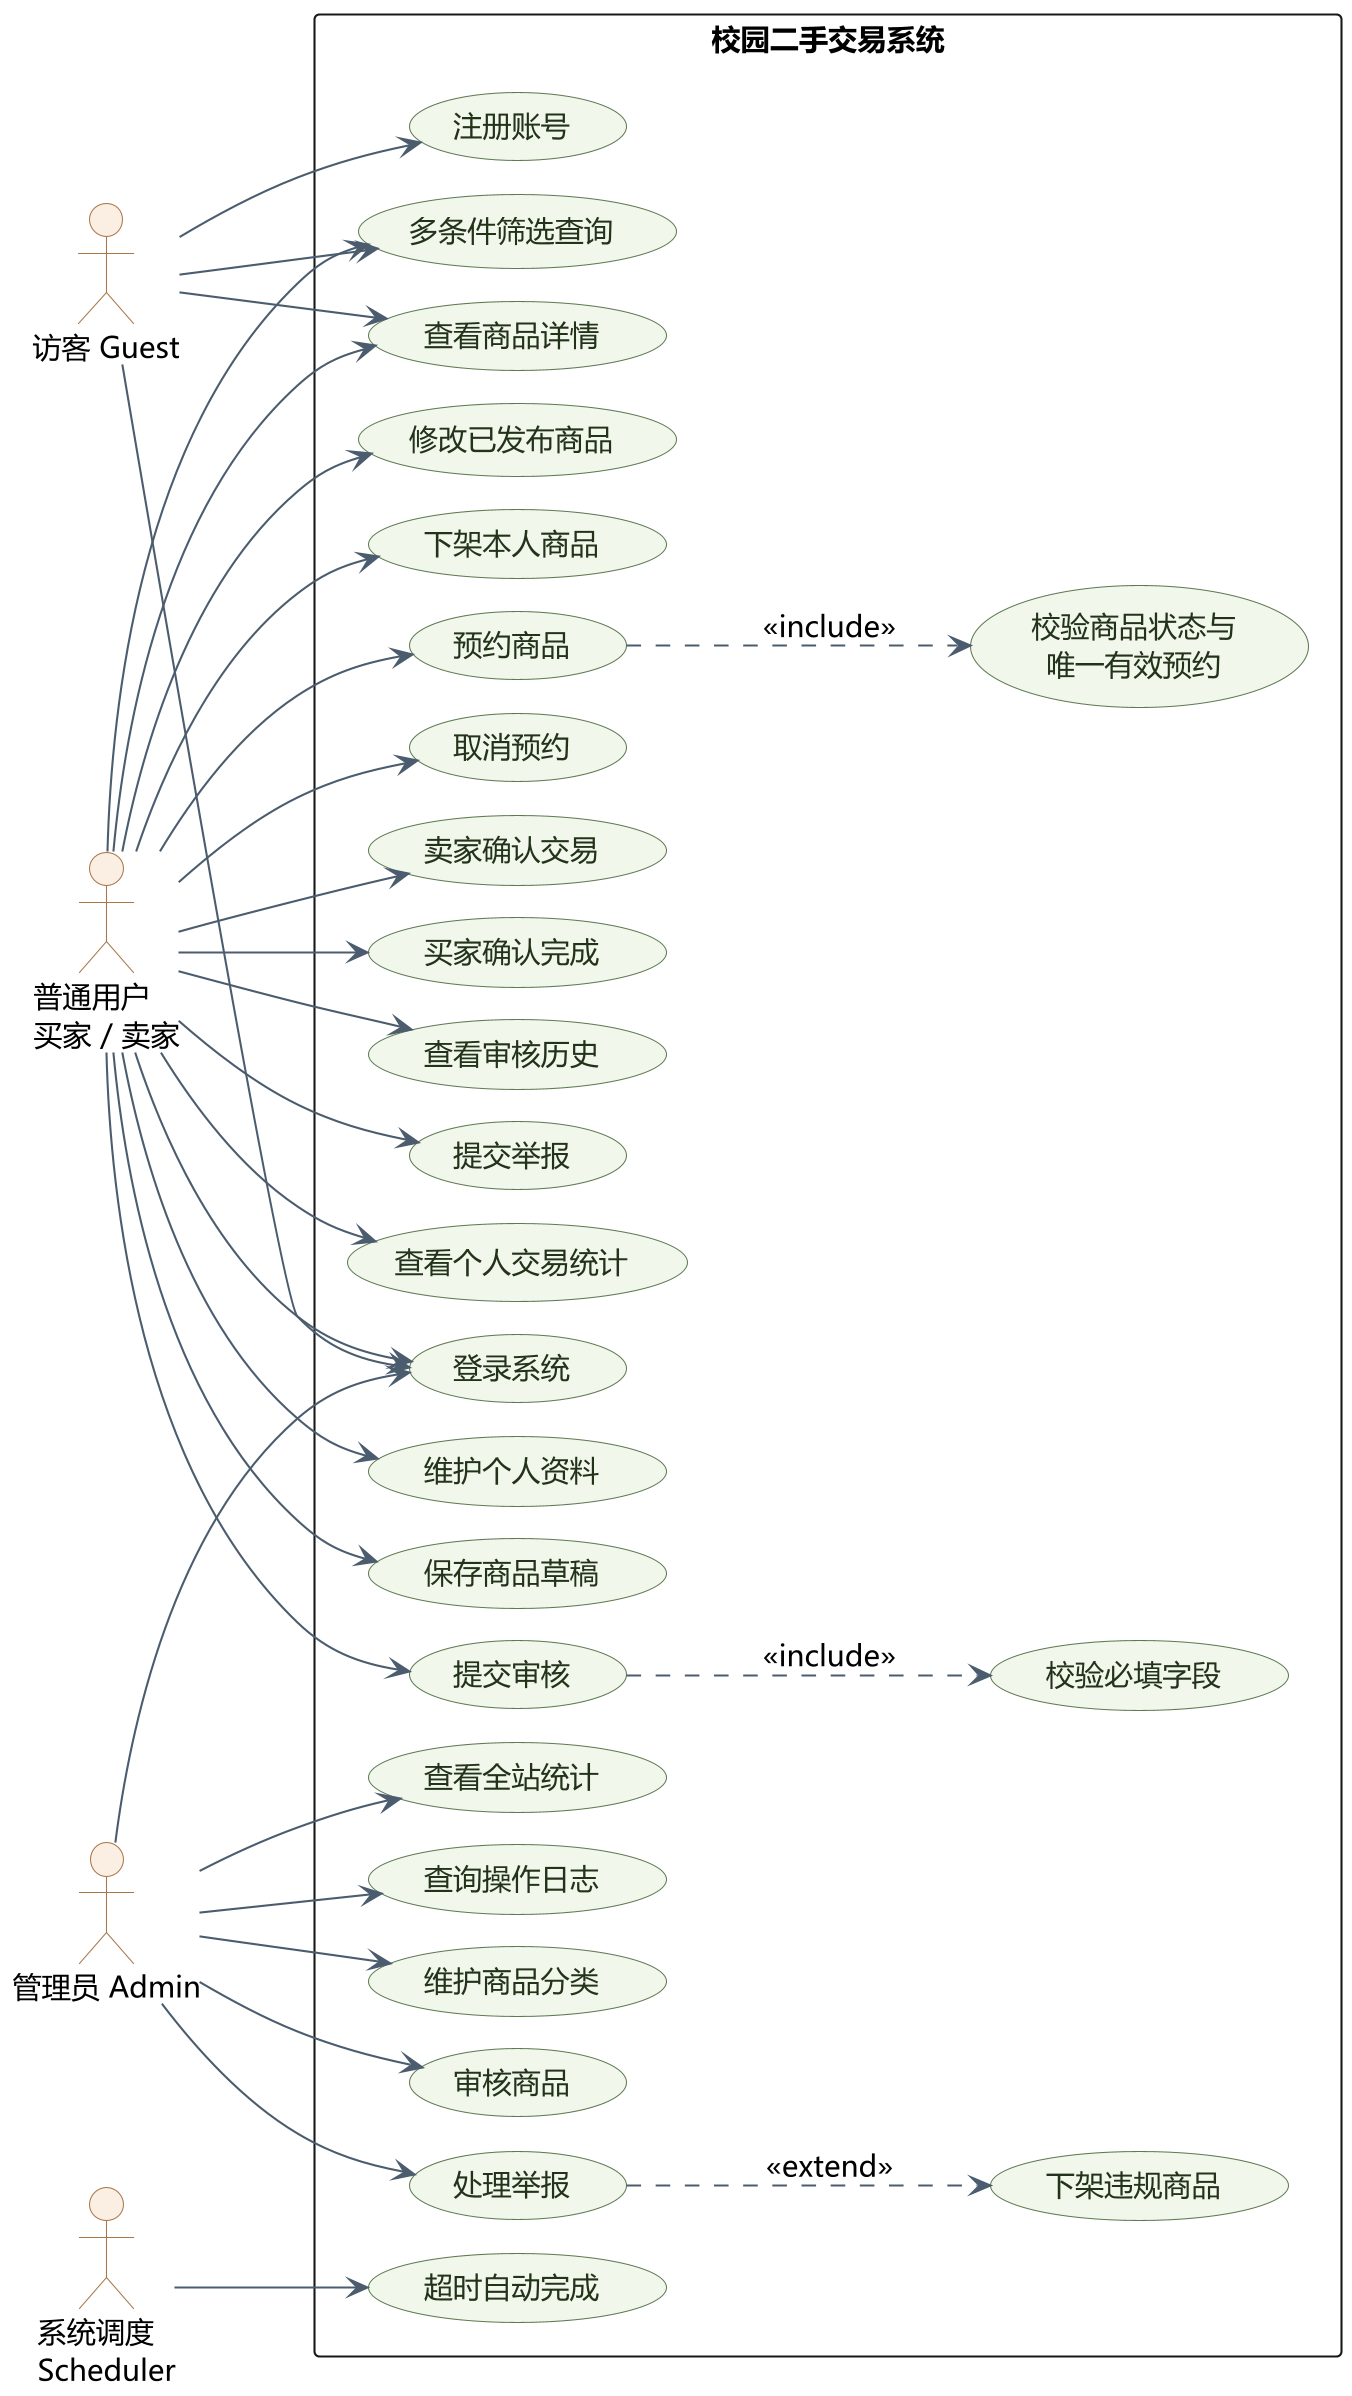
\includegraphics[width=0.54\textwidth]{uml3.png}
\par\vspace{2pt}
\captionof{figure}{校园二手交易系统用例图}\label{fig:uml3}
\end{minipage}
\end{center}

用例图定义四类参与者与 25 个用例。访客可注册、登录、筛选查询与查看详情；普通用户同时是买家和卖家，用例覆盖发布、修改、下架、预约、取消、确认、举报与本人统计；管理员负责审核、举报处置、分类维护、全站统计与日志；系统调度不是人，唯一用例是超时自动完成。

图中标注两个包含关系与一个扩展关系：提交审核包含校验必填字段；预约商品包含校验商品状态与唯一有效预约（并发、重复提交、旧页面、本人商品四个异常都在此判定）；处理举报扩展出下架违规商品。用例图的作用是把 REQ-016 的权限边界画清楚——管理员的用例没有一条连到普通用户，普通用户的用例也没有连到审核与全站统计。

\clearpage
\subsection{行为性图（二）：活动图}

\begin{center}
\begin{minipage}{\textwidth}\centering
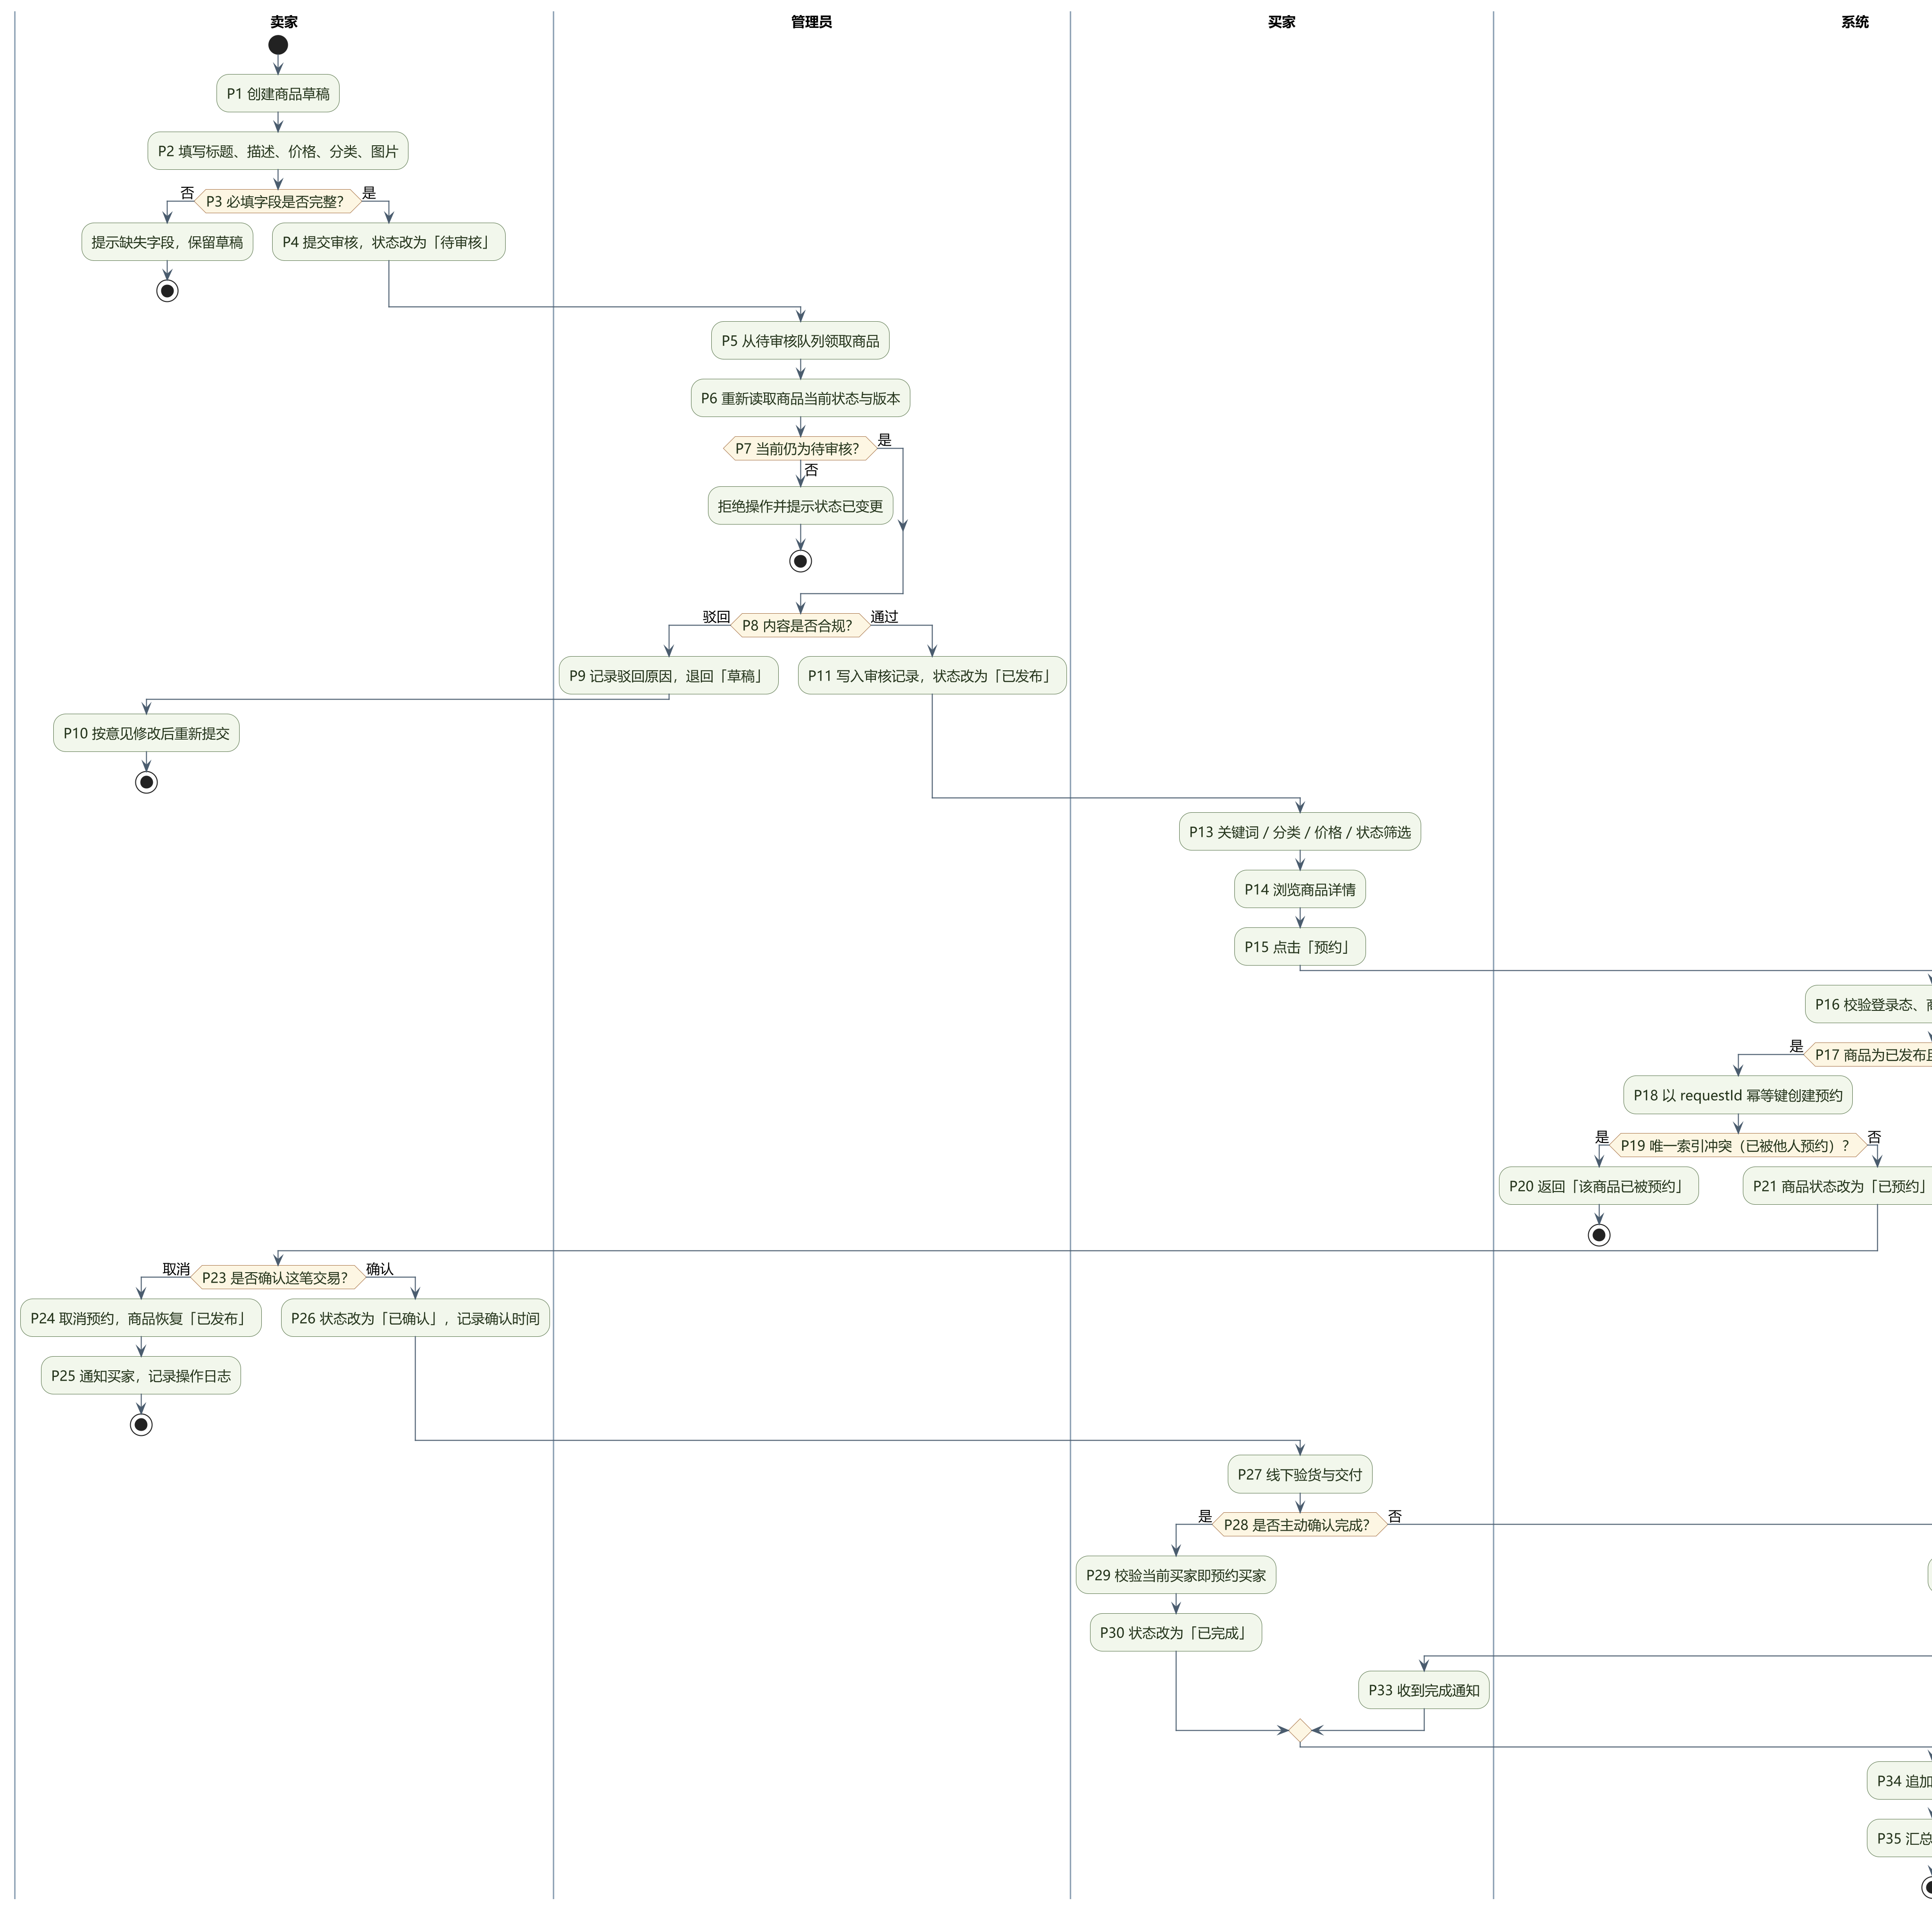
\includegraphics[width=0.96\textwidth]{uml4.png}
\par\vspace{2pt}
\captionof{figure}{商品从发布到完成的主流程活动图（P1--P35）}\label{fig:uml4}
\end{minipage}
\end{center}

活动图用卖家、管理员、买家、系统四条泳道展开完整的交易生命周期，动作编号 P1--P35 便于引用。三个分支直接对应实验一的异常处理：\textbf{P3} 必填字段不完整则保留草稿并终止；\textbf{P7} 管理员领取商品后必须重新读取状态，否则拒绝操作（REQ-003 并发冲突）；\textbf{P17 / P19} 预约的两道闸门，先判“已发布且非本人商品”，再靠唯一索引判并发，失败是显式终止路径而不是异常。

把“系统”单列一条泳道，是因为自动完成容易被误认为由用户触发，从而在实现时漏掉定时任务；P31/P32 放在系统泳道，可直接对应组件图中的定时调度组件。

\clearpage
\subsection{行为性图（三）：状态图}

\begin{center}
\begin{minipage}{\textwidth}\centering
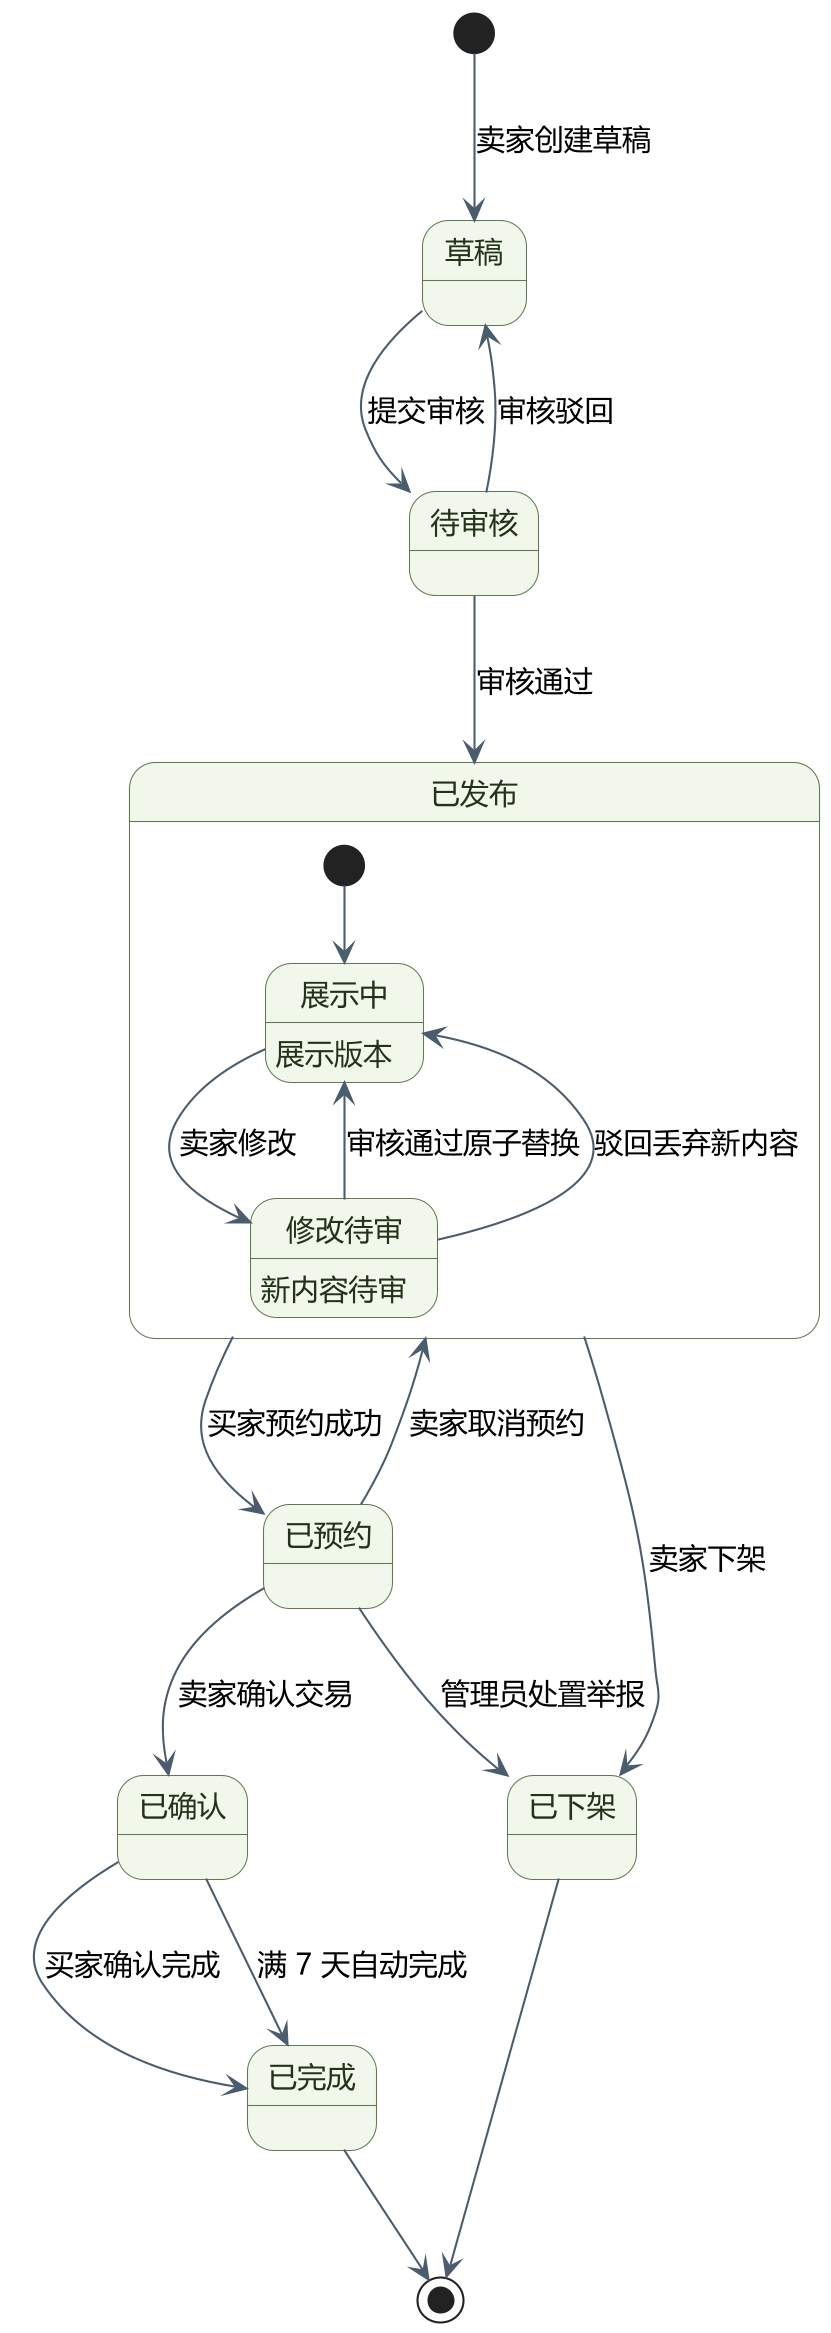
\includegraphics[width=0.34\textwidth]{uml5.png}
\par\vspace{2pt}
\captionof{figure}{商品状态机（含“已发布”组合状态）}\label{fig:uml5}
\end{minipage}
\end{center}

状态图把实验一的状态表图形化，并新增组合状态“已发布”，内部含“展示中”与“修改待审”两个子状态。

之所以用组合状态而不是新增第八个状态，是因为一旦新增，“商品是否可被查询到”“是否可被预约”“统计算不算已发布”三处判断都要同时改，驳回后还要记住原状态。用组合状态后对外可见状态始终是“已发布”，待审内容只是附属对象，通过时原子替换、驳回时直接丢弃。

图中刻意没有画“已完成 $\rightarrow$ 已预约”“已下架 $\rightarrow$ 已发布”，实验一明确禁止这些转换，用“不画”表达禁止比画一条打叉的线更清晰：从已完成与已下架只有指向终态的转移。

\clearpage
\subsection{交互性图：时序图}

\begin{center}
\begin{minipage}{\textwidth}\centering
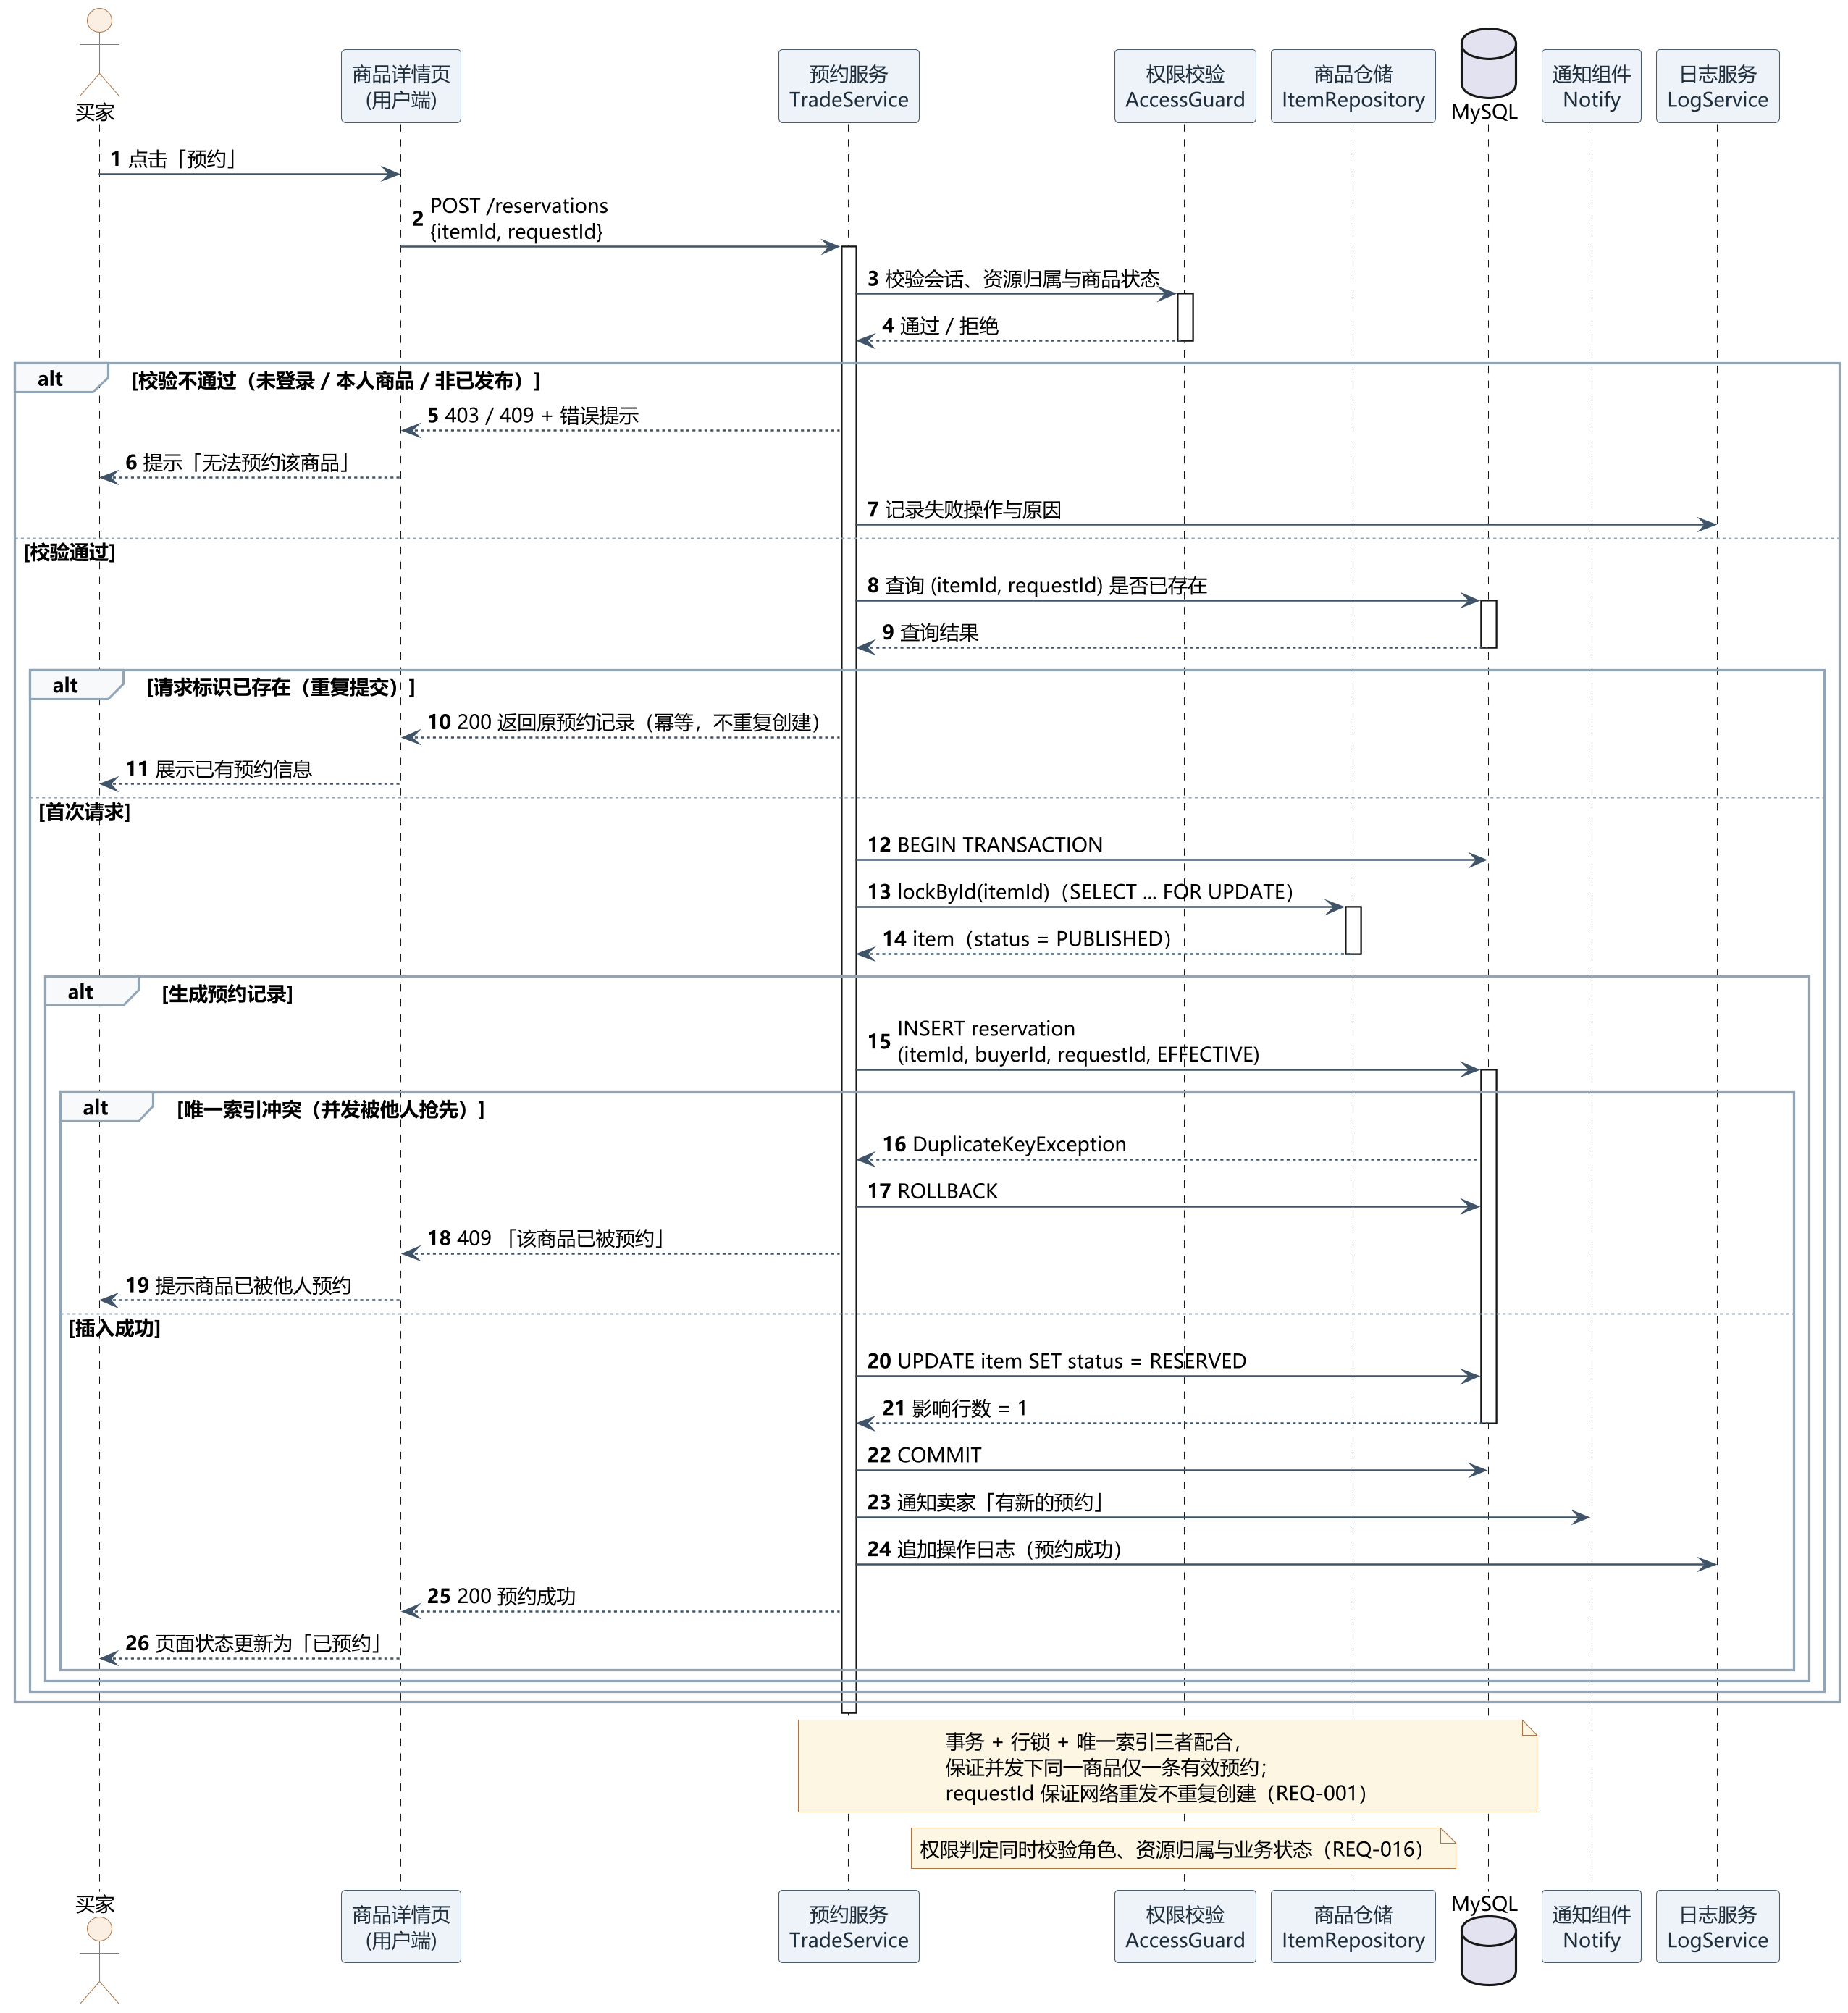
\includegraphics[width=0.84\textwidth]{uml6.png}
\par\vspace{2pt}
\captionof{figure}{商品预约时序图（含幂等与并发控制）}\label{fig:uml6}
\end{minipage}
\end{center}

时序图选择全系统最复杂的动作——预约，8 条生命线、26 条消息、三层嵌套分支。

\begin{enumerate}[leftmargin=2em,itemsep=1pt]
  \item \textbf{先鉴权后业务}：同时检查会话、商品归属与商品状态，任一不满足即返回 403/409，失败也要写日志——预约本人商品、旧页面预约已成交商品本身需要留痕。
  \item \textbf{幂等查重前置}：以 (itemId, requestId) 查重，命中直接返回原记录。必须在加锁之前完成，否则重复请求会排队等锁。
  \item \textbf{事务内加锁插入}：开事务后对商品行加锁再插入，唯一索引冲突则回滚返回“已被预约”，成功则更新商品状态后提交。行锁、唯一索引、事务缺一不可：只有唯一索引无法区分“重复提交”与“别人抢先”，只有行锁则重发仍会重复创建。
\end{enumerate}

实验一的两条验收标准在此一一对应：并发只留一条有效记录对应唯一索引冲突分支，重发记录数不增加对应幂等分支。
